\subsection{Opis hipotezy}\label{opis-hipotezy}

\textbf{Numer:} 5\\\textbf{Nazwa:} Alkohol we krwi kierowcy a
czas\\\textbf{Treść:} Częściej wypadki spowodowane obecnością alkoholu
we krwi kierowcy będą zdarzać się w okolicach świąt, wieczorami i w
weekendy.

\subsection{Wyniki związane z
hipotezą}\label{wyniki-zwiazane-z-hipoteza}

\centerline{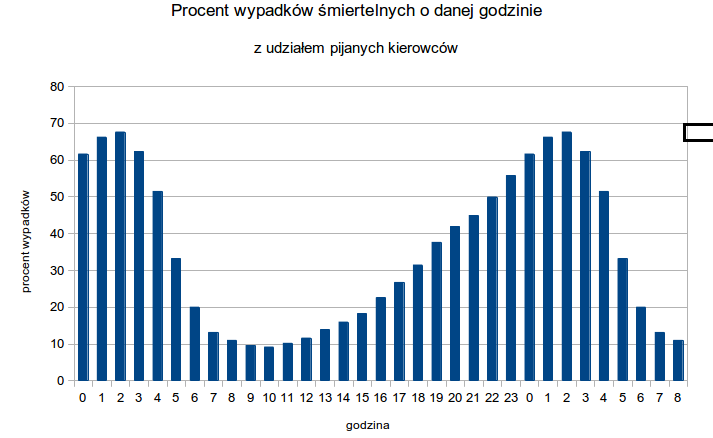
\includegraphics[width=0.8\textwidth]{images/hipotheses/drunk_drivers/hour.png}}

\centerline{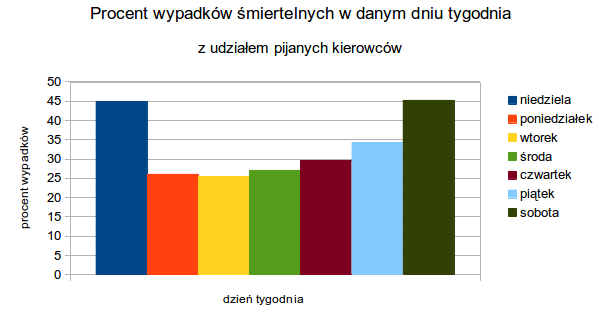
\includegraphics[width=0.8\textwidth]{images/hipotheses/drunk_drivers/day_of_week.png}}

\centerline{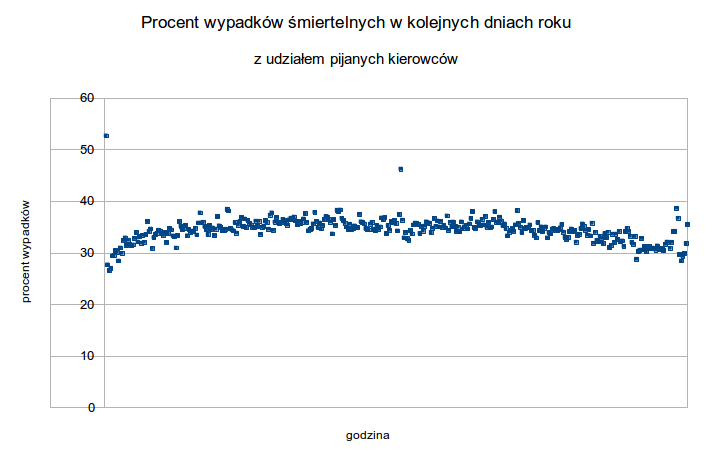
\includegraphics[width=0.8\textwidth]{images/hipotheses/drunk_drivers/day_of_year.png}}

\subsection{Weryfikacja i wnioski}\label{weryfikacja-i-wnioski}

Postawiona hipoteza sprawdziła się. Wyraźny wzrost procentowego udziału
wypadków spowodowanych przez pijanych kierowców obserwujemy w weekend -
zarówno w sobotę jak i w niedzielę jest to ok. 45\% a więc bardzo wysoka
wartość.

Patrząc na rozkład godzinny, widzimy wyraźny stały wzrost aż do godziny
2 gdzie wartość osiąga maksimum w okolicach bardzo wysokiej wartości
68\%, który następnie gwałtownie spada aż do minimum w godzinach
porannych (8 - 10).

W ciągu roku najbardziej wybija się 1 stycznia z wartością ponad 50\%
oraz święto niepodległości 4 lipca (47\%). Nieznaczny wzrost notujemy
również pod koniec roku, w okolicach świąt Bożego Narodzenia.
